\section{Auswertung}
\begin{table} 
\centering 
\caption{Messwerte der Zeitparameter a und b, Kondensator- und Generatorspannung, sowie die errechnete Phasendifferenz in Abhängigkeit von der Frequenz $\nu$.} 
\label{tab: frequenzabhängigkeit} 
\begin{tabular}{S S S S S S } 
\toprule  
{$\nu$ / \si{\hertz}} & {$U$ / $\si{\volt}$} & {$U_C$ / $\si{\volt}$} & {$a$ / $\si{\micro\second}$} & {$b$ / $\si{\micro\second}$} & {$\phi$ / rad}  \\ 
\midrule  
 10  & 4.64  & 4.64  & 0.00  & 100000.00  & 0.00\\ 
25  & 4.64  & 4.64  & 0.00  & 40000.00  & 0.00\\ 
500  & 4.64  & 4.60  & 0.00  & 2000.00  & 0.00\\ 
1000  & 4.64  & 4.64  & 0.00  & 1000.00  & 0.00\\ 
5000  & 4.68  & 4.80  & 0.00  & 200.00  & 0.00\\ 
5500  & 4.72  & 4.84  & 0.00  & 180.00  & 0.00\\ 
6000  & 4.80  & 4.84  & 1.10  & 167.00  & 0.04\\ 
6500  & 4.80  & 4.88  & 1.10  & 153.00  & 0.05\\ 
7000  & 4.72  & 4.92  & 1.20  & 142.00  & 0.05\\ 
25000  & 4.56  & 9.20  & 3.16  & 40.00  & 0.50\\ 
26000  & 4.60  & 9.88  & 3.44  & 38.48  & 0.56\\ 
27000  & 4.60  & 10.80  & 3.76  & 36.92  & 0.64\\ 
28000  & 4.48  & 11.80  & 4.18  & 35.75  & 0.73\\ 
29000  & 4.44  & 12.90  & 3.56  & 34.48  & 0.65\\ 
30000  & 4.48  & 14.10  & 4.06  & 33.30  & 0.77\\ 
31000  & 4.44  & 15.30  & 6.71  & 32.20  & 1.31\\ 
32000  & 4.46  & 16.40  & 6.71  & 31.26  & 1.35\\ 
33000  & 4.32  & 17.00  & 6.40  & 30.27  & 1.33\\ 
34000  & 4.32  & 16.90  & 7.36  & 29.46  & 1.57\\ 
35000  & 4.32  & 15.90  & 9.32  & 28.50  & 2.05\\ 
36000  & 4.36  & 14.60  & 9.80  & 27.85  & 2.21\\ 
37000  & 4.40  & 13.00  & 10.30  & 26.95  & 2.40\\ 
38000  & 4.48  & 11.50  & 10.50  & 26.32  & 2.51\\ 
39000  & 4.48  & 10.30  & 9.72  & 25.64  & 2.38\\ 
40000  & 4.52  & 9.04  & 9.80  & 24.92  & 2.47\\ 
41000  & 4.56  & 8.08  & 10.40  & 24.38  & 2.68\\ 
42000  & 4.52  & 7.32  & 10.30  & 23.92  & 2.71\\ 
43000  & 4.56  & 6.60  & 9.70  & 23.24  & 2.62\\ 
44000  & 4.56  & 6.00  & 9.40  & 22.74  & 2.60\\ 
45000  & 4.60  & 5.48  & 9.60  & 22.27  & 2.71\\ 
\bottomrule 
\end{tabular} 
\end{table}
\begin{table} 
\centering 
\caption{Zeitlicher Verlauf der Amplitude des gedämpften Schwingkreises} 
\label{tab: amplitude} 
\begin{tabular}{S S } 
\toprule  
{$t$ / $10^{-5}\si{\second}$} & {$A$ / $\si{\volt}$}  \\ 
\midrule  
 0.0  & 9.84\\ 
3.0  & 9.04\\ 
6.0  & 8.40\\ 
9.0  & 7.92\\ 
12.0  & 7.52\\ 
15.0  & 7.12\\ 
18.0  & 6.80\\ 
21.0  & 6.56\\ 
24.0  & 6.16\\ 
27.0  & 5.92\\ 
30.0  & 5.76\\ 
33.0  & 5.68\\ 
36.0  & 5.52\\ 
\bottomrule 
\end{tabular} 
\end{table}


\begin{figure}
  \centering
  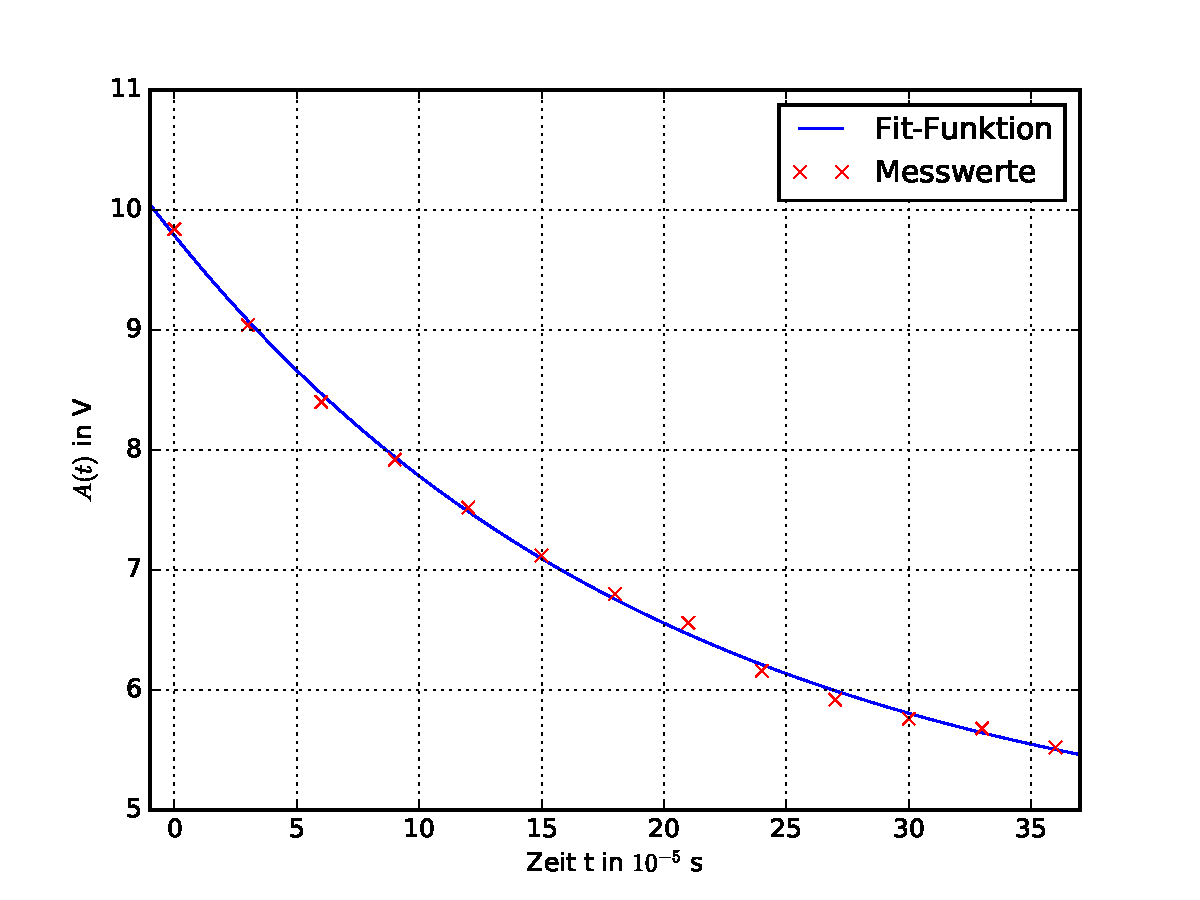
\includegraphics[width = \textwidth]{../Messdaten/amplitude.pdf}
  \caption{Zeitlicher Verlauf der Amplitude (unter Anwendung des Logarithmus) des gedämpften Schwingkreises und Regressiongerade.}
  \label{fig: amplitude}
\end{figure}

\subsection{Frequenzabhängigkeit der Kondensatorspannung}
Die gemessenen Werte der Generator- und Kondensatorspannung unter variabler Frequenz sind in Tabelle \ref{tab: frequenzabhängigkeit} aufgeführt.
Hierbei ist zu erkennen, dass bei den ersten neun Messwerten, die in kleinen Frequnezbereichen aufgenommen wurden, nur eine geringfügige
Diskrepanz zwischen beiden Größen besteht. Die graphische Darstellung der Werte bei höheren Frequenzen ist in Abbildung \ref{fig: spannungsverlauf_U_C}
einzusehen. Für die Resonanzfrequenz entnimmt man aus der Messreihe den Wert:
\begin{equation}
  \nu_{0, exp} = \SI{33}{\kilo\hertz}.
  \label{eq: exp_resonanzfrequenz}
\end{equation}
Gemäß Formel \eqref{eq:} berechnet sich der Theoriewert der Resonanzfrequenz $\nu_{0, th}$, sowie die prozentuale Abweichung $d_{\nu}$ des gemessenen Wertes zu:
\begin{align}
  \nu_{0, th} &= \SI{3.409e4}{\hertz} \\
  d_{\nu} &= \SI{-3.19}{\percent}.
\label{eq: theo_resonanzfrequenz}
\end{align}
Des Weiteren entnimmt man aus der graphischen Darstellung die Größen $\nu_+$ und $\nu_-$, aus denen die Breite (...) bestimmt werden kann.
\begin{align}
  \nu_{+} &= \SI{3.745e4}{\hertz} \\
  \nu_{-} &= \SI{2.860e4}{\hertz} \\
  (\nu_{+}-\nu_{-})_{exp} &= \SI{8.85e3}{\hertz}.
\label{eq: breite_exp}
\end{align}
Für den Theoriewert der Breite [gemäß \eqref{}] und die prozentuale Abweichung ergeben sich hieraus:
\begin{align}
  (\nu_{+}-\nu_{-})_{th} &= \SI{8.02e3}{\hertz}\\
  d_{\nu_{+}-\nu_{-}} &= \SI{10.34}{\percent}.
\label{eq: theo_breite}
\end{align}

\begin{figure}
  \centering
  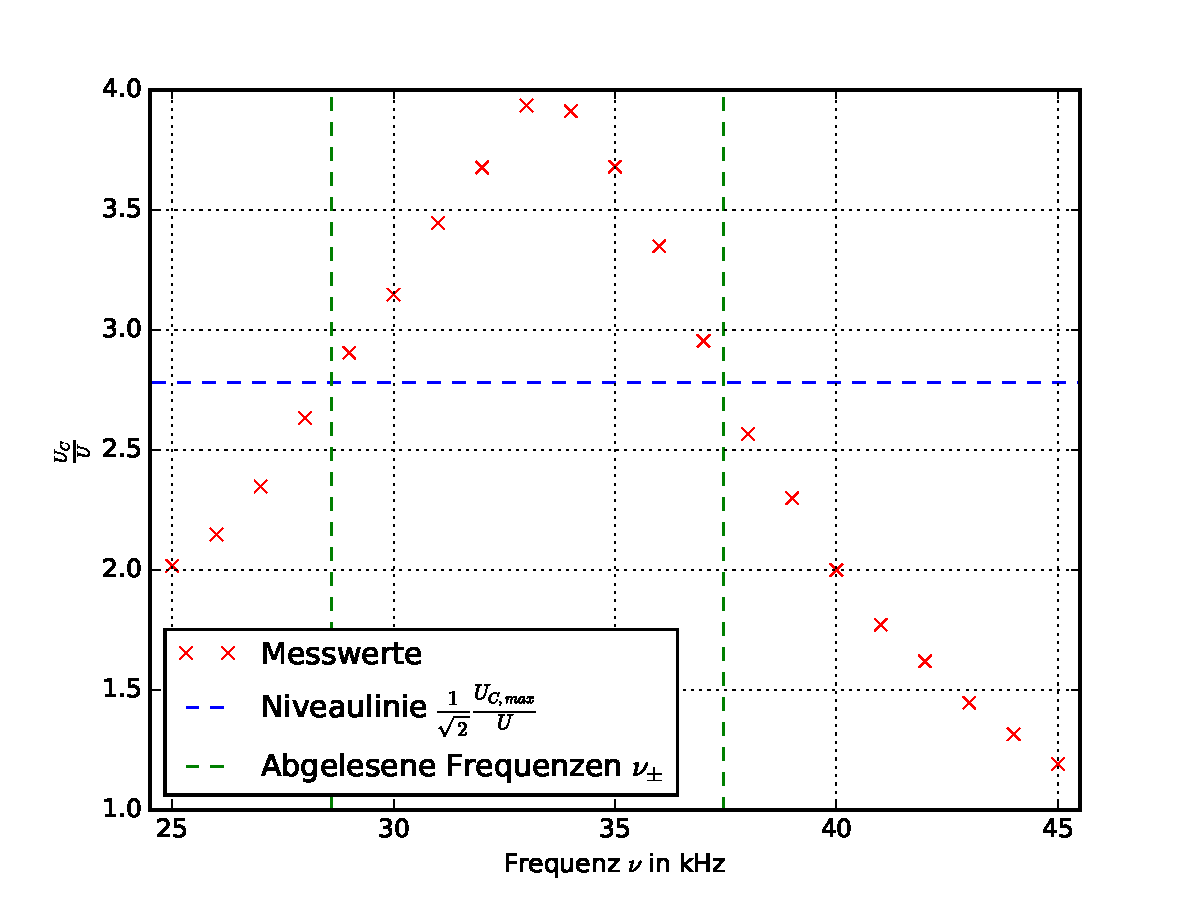
\includegraphics[width = \textwidth]{../Messdaten/U_f_linear.pdf}
  \caption{Verlauf der Spannung am Kondensator unter variabler Frequenz, sowie eingezeichnete Hilfslinien zum Ablesen der relevanten Größen.}
  \label{fig: spannungsverlauf_U_C}
\end{figure}

\begin{figure}
  \centering
  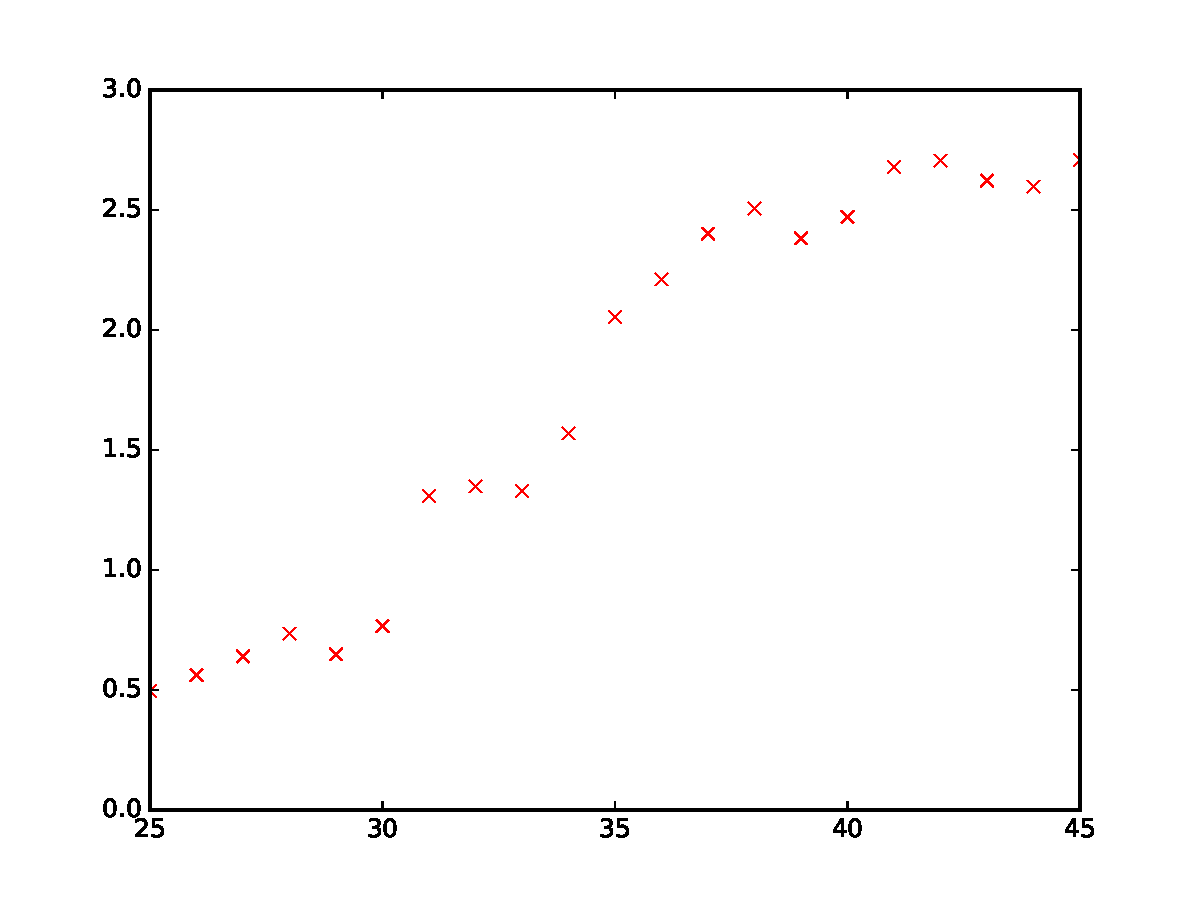
\includegraphics[width = \textwidth]{../Messdaten/phase_f_linear.pdf}
  \caption{Verlauf der Phasendifferenz zwischen Erreger- und Kondensatorspannung unter variabler Frequenz.}
  \label{fig: phasenverlauf}
\end{figure}
